% =========================================================
% SECTION 3.6: RE-RANKING (LÝ THUYẾT)
% =========================================================
\section{Xếp hạng văn bản (Re-ranking)}
\label{sec:reranking}

\subsection{Định nghĩa}
Xếp hạng văn bản (\textit{Re-ranking}) là kỹ thuật tinh chỉnh kết quả tìm kiếm, thường được áp dụng trong giai đoạn hai của các hệ thống truy xuất thông tin nhiều tầng. Trong kiến trúc này, sau khi một tập hợp các tài liệu ứng viên được truy xuất sơ bộ bởi các thuật toán tìm kiếm tốc độ cao (như tìm kiếm vector hoặc từ khóa), mô hình Re-ranking sẽ được sử dụng để đánh giá lại mức độ phù hợp của từng tài liệu đối với câu truy vấn một cách chi tiết hơn.

Về mặt kỹ thuật, các mô hình xếp hạng hiện đại thường dựa trên kiến trúc \textbf{Cross-Encoder}. Khác với \textbf{Bi-Encoder} (vốn mã hóa truy vấn và văn bản thành hai vector độc lập), Cross-Encoder tiếp nhận đầu vào là cặp dữ liệu (truy vấn, văn bản) đồng thời. Mô hình sử dụng cơ chế sự chú ý (\textit{Self-Attention}) trong mạng nơ-ron Transformer để phân tích mối quan hệ tương tác ngữ nghĩa giữa từng từ của câu truy vấn với toàn bộ nội dung văn bản, từ đó xuất ra một điểm số tương đồng (\textit{relevance score}) duy nhất \cite{nogueira2019passage}.

\begin{figure}[h]
    \centering
    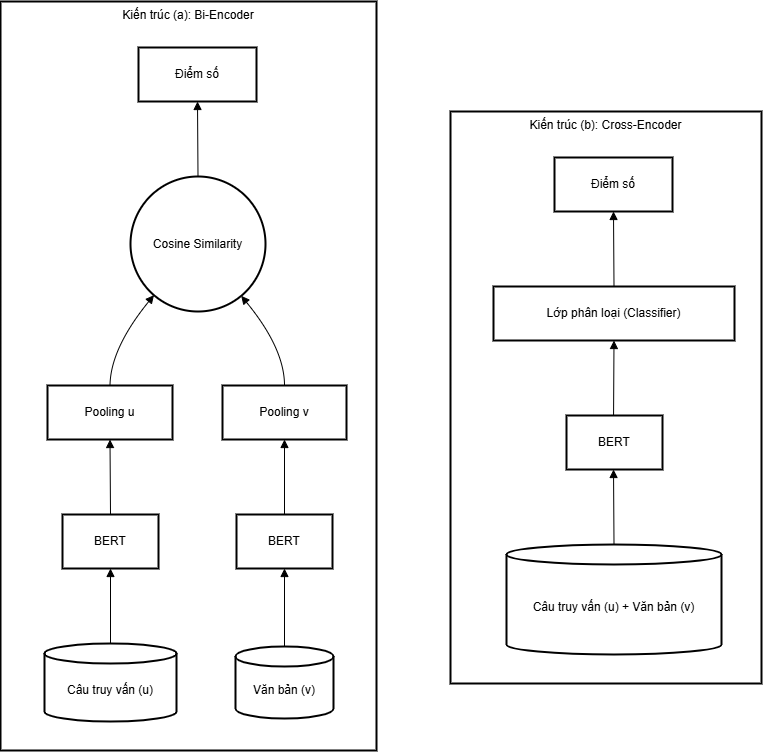
\includegraphics[width=0.8\textwidth]{images/so sanh.png}
    \caption{So sánh kiến trúc Bi-Encoder và Cross-Encoder}
    \label{fig:cross_bi_encoder}
\end{figure}

\subsection{Vai trò trong hệ thống truy xuất}
Trong bài toán truy xuất thông tin, luôn tồn tại sự đánh đổi giữa độ phủ (\textit{Recall}) và độ chính xác (\textit{Precision}). Các phương pháp truy xuất vector thường ưu tiên độ phủ để đảm bảo không bỏ sót thông tin, dẫn đến việc tập kết quả trả về có thể chứa nhiều tài liệu nhiễu hoặc không sát nghĩa.

Việc tích hợp Re-ranking đóng vai trò như một bộ lọc ngữ nghĩa cao cấp. Nhờ khả năng ``đọc hiểu'' sâu sắc mối quan hệ giữa câu hỏi và văn bản, Re-ranking giúp loại bỏ các kết quả dương tính giả (\textit{false positives}) và sắp xếp các tài liệu thực sự hữu ích lên vị trí đầu tiên. Các nghiên cứu thực nghiệm đã chứng minh rằng kiến trúc ``Truy xuất rồi Xếp hạng lại'' (\textit{Retrieve-then-Rerank}) mang lại hiệu suất vượt trội trên các bảng xếp hạng đánh giá truy xuất thông tin, đặc biệt trong các trường hợp truy vấn đòi hỏi khả năng suy luận phức tạp hoặc miền dữ liệu đặc thù \cite{thakur2021beir}.